\documentclass{standalone}


\usepackage{tikz}
\usetikzlibrary {calc} 

\begin{document}
	
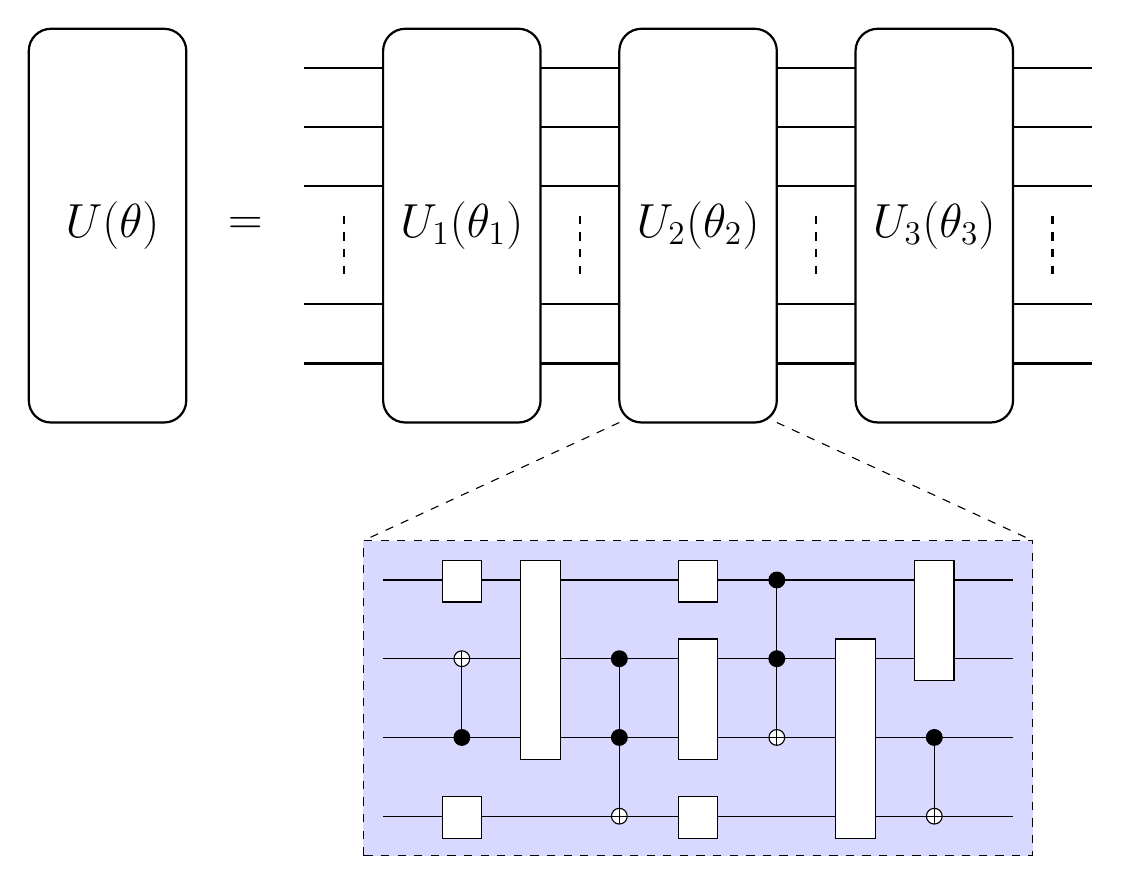
\begin{tikzpicture}
%	\draw (2,0) -- (-1,2);
%	\draw (0,0) circle [radius=10pt];
%	\draw  [<->](0,0.25) -- (0.5,1.2);
%	\draw (0,0) rectangle (0.5,1);
%	\draw[step=.5cm] (-2,-2) grid (2,2);
%   \draw [<->] (0,0) arc [start angle=180, end angle=30, radius=10pt];
%	\tikz \foreach \x in {3,5,7}
%		\draw (\x,0) rectangle (\x,2);
%\draw[thick,rounded corners=8pt]
%										(0,0) -- (2,1);

	\draw[thick,rounded corners=8pt,fill=white] (-1.5,0) rectangle (0.5,5);
	
	\node [anchor=center] at (-1.75/4,2.5) {\LARGE $U(\theta)$};
	
	\node [anchor=center] at (1.25,2.5) {\LARGE $=$};

	\foreach \x [evaluate=\x] in {3,6,9,12} 
		\draw[thick,dash pattern=on 3pt off 3pt] (\x-0.5,0.75*3.5) -- (\x-0.5,0.75*2.5);

	\foreach \x [evaluate=\x] in {3,6,9} {
		\foreach \y in {1,2,4,5,6}
			\draw[thick] (\x-1,0.75*\y) -- (\x+3,0.75*\y);
		}

	\foreach \x  [evaluate=\x] in {1,2,3} {
		\draw[thick,rounded corners=8pt,fill=white] (3*\x,0) rectangle (3*\x+2,5);
		\node [anchor=center] at (3*\x+1,2.5) { \LARGE $U_\x(\theta_\x)$};
	}

	\draw[dashed]  (6,0) -- (2.75,-1.5);
	\draw[dashed]  (8,0) -- (11.25,-1.5);

	

\begin{scope}[shift={(3,-5)}]
	
	\draw[dashed,fill=blue!15] (-0.25,-.5) rectangle (8.25,3.5);

	\tikzset{pics/cnot/.style n args={2}{
		code = {
			\draw[thin,fill=white] (0,#1) circle (0.1cm);
			\draw[thin] (0,#1) -- +(0.1,0);
			\draw[thin] (0,#1) -- +(0,0.1);
			\draw[thin] (0,#1) -- +(-0.1,0);
			\draw[thin] (0,#1) -- +(0,-0.1);
			\draw[thin] (0,#1) -- +(0.1,0);
%			
			\draw[thin,fill=black] (0,#2) circle (0.1cm);
			\draw[thin] (0,#1) -- (0,#2);
				}
	}}

	\tikzset{pics/ccnot/.style n args={2}{
		code = {
			\draw[thin,fill=white] (0,#1) circle (0.1cm);
			\draw[thin] (0,#1) -- +(0.1,0);
			\draw[thin] (0,#1) -- +(0,0.1);
			\draw[thin] (0,#1) -- +(-0.1,0);
			\draw[thin] (0,#1) -- +(0,-0.1);
			\draw[thin] (0,#1) -- +(0.1,0);
			%
			\draw[thin,fill=black] (0,#2+1) circle (0.1cm);
			\draw[thin] (0,#1) -- (0,#2+1);
			\draw[thin,fill=black] (0,#2) circle (0.1cm);
%			\draw[thin] (0,#1) -- (0,#2);
		}
	}}


	\tikzset{pics/onequbit/.style n args={0}{
		code = {
			\draw[thin,fill=white] (-0.5+0.25,-0.5+0.22) rectangle (0.5-0.25,0.5-0.25);
		}
	}}

	\tikzset{pics/twoqubit/.style n args={0}{
		code = {
			\draw[thin,fill=white] (-0.5+0.25,-0.5+0.22) rectangle (0.5-0.25,1.5-0.25);
		}
	}}

	\tikzset{pics/threequbit/.style n args={0}{
		code = {
			\draw[thin,fill=white] (-0.5+0.25,-0.5+0.22) rectangle (0.5-0.25,2.5-0.25);
		}
}}

%	let \p1=(0.25,0.25);
		
	\foreach \x [evaluate=\x] in {1,2,3} {
		\foreach \y [evaluate=\x] in {0,...,3} 
		\draw[thin] (\x-1,\y) -- (\x+5,\y);
	}

	% first layer
	\draw (1,0) pic {onequbit};
	\draw (1,0) pic {cnot={2}{1})};
	\draw (1,3) pic {onequbit};
	
	% second layer
	\draw (2,1) pic {threequbit};
 

	
	% third layer
%	\pic (1,1) {oplus=4};
%	\draw[thin,fill=white] (2.25,-0.5+1) rectangle (2.25+0.75,1.5+1-0.25/4);
	
	% forth layer
%	\draw[thin,fill=white] (3.25,2.5+0.25/4) rectangle (3.25+0.75,3.5-0.25/4);
	
	\draw (3,0) pic {ccnot={0}{1})};
		
	% fifth layer 
	\draw (4,1) pic {twoqubit};
	\draw (4,0) pic {onequbit};
	\draw (4,3) pic {onequbit};
	
	% fifth layer 
	\draw (5,0) pic {ccnot={1}{2})};
	
	% sixth layer
	
	\draw (6,0) pic {threequbit};
	
	% seventh layer 
	\draw (7,0) pic {cnot={0}{1})};
	\draw (7,2) pic {twoqubit};


	
%	\draw[thin,rounded corners=2pt,fill=white] (0,-0.5) rectangle (1,-2.25);
%	\draw[thin,rounded corners=2pt,fill=white] (1.5,1) rectangle (2.5,-1);
		

\end{scope}

\end{tikzpicture}
\end{document}